\section{Implementation}

The first step was to create or find an environment that with an accurate depiction or an environment wrapping around the pokemon game itself. After finding the environment, the details of the environment had to be checked ensure compatible with different algorithms intended to be used. Once an environment and RL algorithm is chosen, a minimum viable product can be achieved by training an agent to play the game and defeat the first gym. After this,  the project can be scaped up by using methods to accelerate the training of the agent without sacrificing the quality of the agent's performance and amount of timesteps it is training for. 

\subsection{Environment}

The implementation of the environment will be broken down into smaller sections that make up the most important aspects of the RL environment. The environment will be implemented using the 'gymnasium' library, which is a popular python library for building RL environments.

The environment to conduct the experiments for this research project was originally written by Peter Whidden and the basis code used for the environment was taken from their github repository and modified to better fit the objectives of the research project. 

\subsubsection*{Reset}

At the start of every episode, the ``reset'' function must be called to reset the environment to its initial state. This is important because the agent must start at the same inital state at the start of every episode to allow for the agent to apply the learnt knowledge from a previous episode to the current one. 

The environment is reset loading the inital game state of the game, which is where the agent starts within the game. This is necessary for this research, as the agent would instead have to go through the process of starting a new game at the start of every episode. In addition, the game requires the player to explore to the next area and return to the starting area before progressing with the game, which would mess with the exploration of the agent. This is because the agent would have already explored the new area however not be rewarded for returning to the same region to find new regions to explore.

After loading in the save state of the game, the ``recent\_screens'' and ``recent\_actions'' would have to be cleared to ensure that the agent is not rewarded for actions that were taken in a previous episode. In addition, other variables that are used to keep track of the state and potential reward such as: ``self.levels\_satisfied'', ``self.base\_explore'', ``self.party\_size"", had to be reset to their default values. 

\subsubsection*{Get Observation}

Get observation takes in the necessary information from the environment and returns it to the agent as the state. First, the function takes in the pixel information of what pyboy is renderinig using ``game\_pixels\_render = self.screen.screen\_ndarray()[:,:,0:1]'' before it is then downscaled by a factor of 2 to make the state space smaller and less RAM intensive. The new ``game\=\_pixels\_render'' is then added to another axis so that it can be compared to the screen information from 2 steps ago. This is compared to the screen information from 2 steps ago to see if the agent has experienced a new screen.

After rendering the screen, the function then takes in the RAM information of the game. This is done by calling ``get\_memory\_value()'' from pyboy to read in the information and assigning it to the necessary variables. RAM values such as: ``level\_sum'', ``badges'', and ``health'' are necessary to be read in from RAM, as they are important to the agent's decision making process and accessible to the player in the game.

\subsubsection*{Step}

The step function is the most important function in the environment, as it is where the agent takes an action from its observation. The chosen action is applied to the emulation before the step function reads in the changes in the emulation and appends it to ``agent\_stats''. The step function then takes in the appended ``agent\_stats'' and uses it to determine the reward for the action. Then it checks if the episode is over if the number of steps has reached its limit before calling the ``get\_observation'' function to get the new state of the environment and the ``step\_counter"" is incremented. At the end, the new observation, the new reward, and if the episode is over is returned to the agent.

\subsection{Reward Function}

The reward function takes in multiple factors when considering the reward to be returned to the agent. However, this specific reward function is designed to be a dense reward function because of how large the search space of the game is. Having a sparse reward function may result in the agent learning at a slower rate and learn to complete the reward tasks instead of the overall objective of the game. Dense reward functions return the agent with more immediate feedback on the selected action and may make learning environment easier. 

The reward function takes in the following factors when considering the reward to be returned to the agent: the number of event flags met, the total level of the pokemon owned, the amount healed by the agent, the number of badges owned, and newly explored screens. Most of the variables updated in the reward function require RAM reading to take in values from the emulation, which has been taken from the datacrystal website \cite{datacrystal}.

A reward has to be assigned for the number of event flags met to assist with guiding the agent to the next objective. This is done by checking if any event flag conditions have been met within the RAM readings of the game and rewarding the agent for every that has been discovered and satisfied. This is necessary because the game has multiple key non-player characters that the agent has to interact with to progress through the game. 

The agent is also rewarded for the total level of the pokemon owned. This is done by taking the sum of levels of the pokemon owned by the agent. This is necessary because the agent has to battle other pokemon and level up its pokemon to become stronger in order to defeat the gym. Therefore, assigning reward to increasing the level of the agents pokemon will reinforce the idea that battling is just as important as exploring. However, the amount of reward the agent can recieve is capped so that it does not become the sole objective of the agent. 

Another reward that is assigned to the agent is the amount healed by the agent. This is done by taking the difference in the health of the pokemon in the previous state and the health in the current state. This is important because the agent recieves a negative reward when losing a battle and is sent back to the starting area. Healing within the game, not only heals the pokemon, allowing it to battle more, but also allows the agent to change the location of where the agent is sent to after losing a battle. This means that the agent would spend less actions returning to the position of where it initially lose the battle.

The agent is also rewarded for the number of badges owned. Normally the agent would be ever increasing this value as it defeats the eight gym leaders in the game. However, for this research the agent only has to recieve a single gym badge before the episode is complete.

\subsection{Navigation}

One issue that arose while training the agent was learning to navigate beyond the starting zone. This was an issue because of the way in which the exploration function was written in the environment. The algorithm would recieve state information through a mixture of screen information and RAM information. The algorithm would then read the screen information and compare the recieved pixel information if it matches or is similar to any previously experienced screen information. Any newly discovered screen information would be rewarded an exploration reward. 

The issue with this method of exploration, within an environment that has to be in sync with the emulation, is that non-static images would give a false positive and reward the agent with exploration due to the new screen information. This was an issue that arose during early training. 

Due to the starting area having some non-static images of moving flowers and water tiles, the agent would be rewarded for staying in the starting area. In addition, the screen images were further varied by the fact that there were randomly moving non-player characters within the same screen. Therefore, the agent was receiving new screen information from the non-static images and moving non-player characters without any action input, which resulted in the agent not learning correctly.

One issue that was encountered while training the agent was getting the agent to increase its confidence with navigating towards the first gym and initiating the battle with the first gym leader. The agent was able to navigate from the starting area at the start of the episode to the zone which held the first gym leader. In addition, the agent was able to swiftly defeat the gym leader, which suggests that it was able to understand battling and the optimum policy to defeat the gym leader the swiftest. However, it had difficulty even navigating within the few tiles around the gym leader. One potential solution to this problem was to increase the reward for completing the first gym, which would indicate to the agent that the gym leader was an important objective and take actions to get there faster. Another solution to this problem would be to increase the discount factor so that the agent was further future sighted and valued high rewarding future states more. 

Another problem that was encountered while training the agent was the agent prioritized exploring the environment over battling, despite having equal scaling for both rewards. This was because the time it took for the agent to efficently explore new areas was less than the time it took for the agent to gain a level from battling. This was because of how sensitive RL is to the reward function. In addition, as the game progresses, the difficulty of exploring new tiles does not increase. However, leveling up the pokemon the agent has in its party becomes harder as the amount of needed experience gained from each battle increases. This was an issue because initially the agent would value battling over exploring as it was performing random movements to view new tiles. However, as the agent got better at exploration, it became more efficient at exploring new tiles than battling. This was an issue because the agent would not be able to defeat the gym leader if it did not have a high enough level pokemon in its party. 

One solution to this problem was to implement a dynamic reward function that would increase and decrease the scale of navigation and battling rewards based on the certain conditions of the agent. One example that was implemented was to increase the reward for battling whenever the agent lost a battle. This would encourage the agent that it needed to prioritize battling over exploring to level up its pokemon to get over the problem and is a very human approach to getting over a problem. 

\subsection{Battling}

Initially, it was assumed that the agent would prioritize battling over exploration as the agent would be rewarded for the total level of the pokemon owned. However, this was not the case as the agent would prioritize exploring the environment over battling. Initially the agent would take random actions and explore the environment while battling when it encountered a wild pokemon. However, as the agent became more experienced navigating the environment to find undiscovered tiles, it deteremined that it could recieve more reward from exploring the environment than battling. This was an issue because the agent would learn to escape and avoid battling to spend more time exploring which would result in the agent not having a high enough level pokemon to defeat the gym leader. 

Due to the agent's policy determining that there is a higher amount of value in choosing to explore instead of battle and the agent's in ability to beyond past a certain point in the game because of its unbattled pokemon, the agent believes that it has found the optimum policy to receive the highest amount of reward given the number of timesteps it has per episode. 

This was solved by increasing the reward for battling and by creating a dynamic reward function. Battling would be encouraged slightly more than exploration, but the amount of reward for battling would be capped when reaching a certain level. This was designed so that the agent would be encouraged to match the level of the pokemon of the gym leader it has to defeat next, which allowed the agent to eventually defeat any pokemon it encounters and unlock more regions of the game and recieve more reward for unsceen tiles.

\subsection{Speeding up agent training}

In order to scale up the project to accelerate the training of the agent, the speed at which the emulation was running was increased. This was done using Pyboy's emulation speed-up function and editing the rate at which screen information and RAM was read to stay in sync with the emulation. This allowed the agent to train at a faster rate, without making any sacrifices to the quality of the agent's training. The emulation was sped up by a rate of 6x because this was the fastest rate at which the environment was able to stay in sync with the emulation. Due to the environment not being a recreation of the original game and instead extract information and applying input to the environment, the environment and emulation had to stay in sync so that information was being extracted and injected at the correct moments.

Another technique used to accelerate the training of the agent was to train the agent in parallel. This was done using the 'SubprocVecEnv' function from the 'stablebaselines3' library. A total of 11 instances of the environment were trained in parallel because this was the maximum amount of instances the hardware used could handle. The hardware used to train the agent is specified in \ref{subsec:Hardware} Hardware Requirements. 11 instances of parallel traning was chosen because it was the maximum amount allowed to be trained on with 64 GB of RAM before the system would crash due to memory issues when updating the policy at the end of every episode. 

\subsection{Memory issues during training}

The length of each episode influenced the amount of RAM needed to be allocated per instance of the environment because the policy would be updated at the end of every episode and the training data for each episode must be stored in RAM. Therefore, the longer the episode the more data needs to be kept within RAM before updating the policy. For the graphs displayed below, the episode length of each episode was set to 2000 steps. %! SAY IF IT WILL BE USED IN THE FINAL FINDINGS OR NOT 

In addition, using gymnasium's 'headless' function allowed the agent to train without the need to render the game, which lowered the system requirements to train. Lowering the hardware requirements to train the agent allows the potential of more instances of the environment to be trained in parallel, which would allow the agent to train at a faster rate.

While training the agent, the hardware component that was bottlenecking further instances of the environment being trained in parallel was the RAM. Training did not have that high of a GPU nor CPU requirement. This is evident in the graphs below. 

\begin{figure}[H]
    \centering
    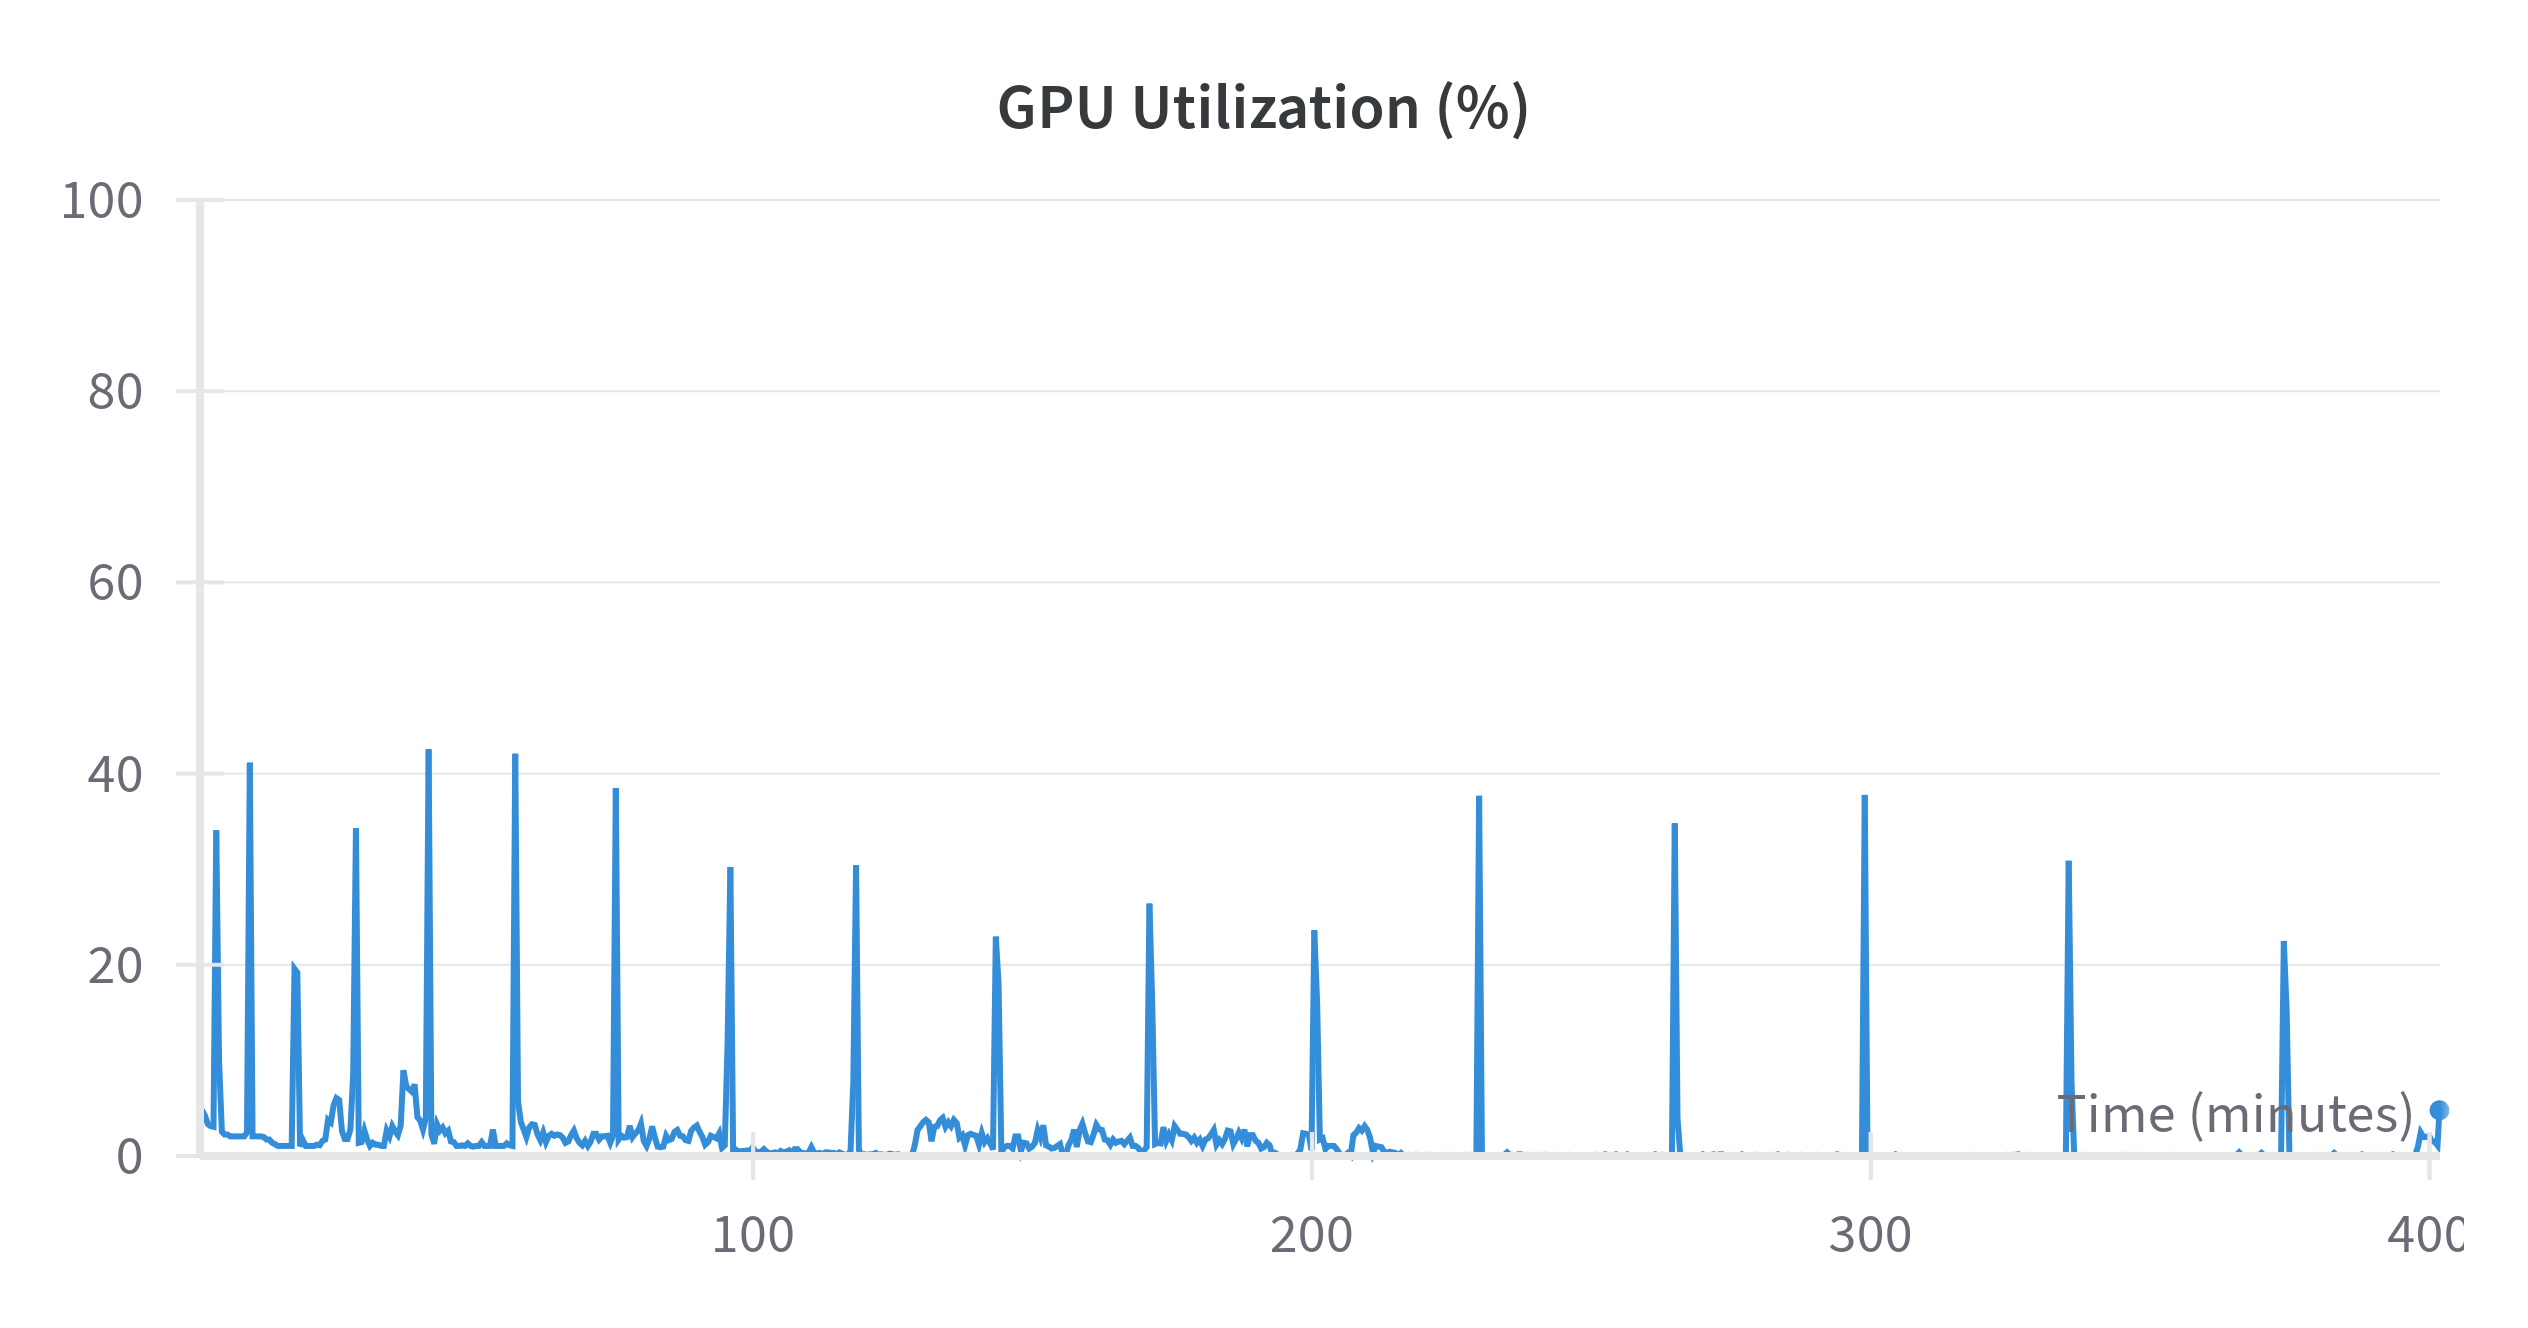
\includegraphics[width=0.8\textwidth]{figures/GPU_Utilization.png}
    \caption{GPU percentage usage while training an agent}
    \label{fig:gpu_memory_usage}
\end{figure}

\begin{figure}[H]
    \centering
    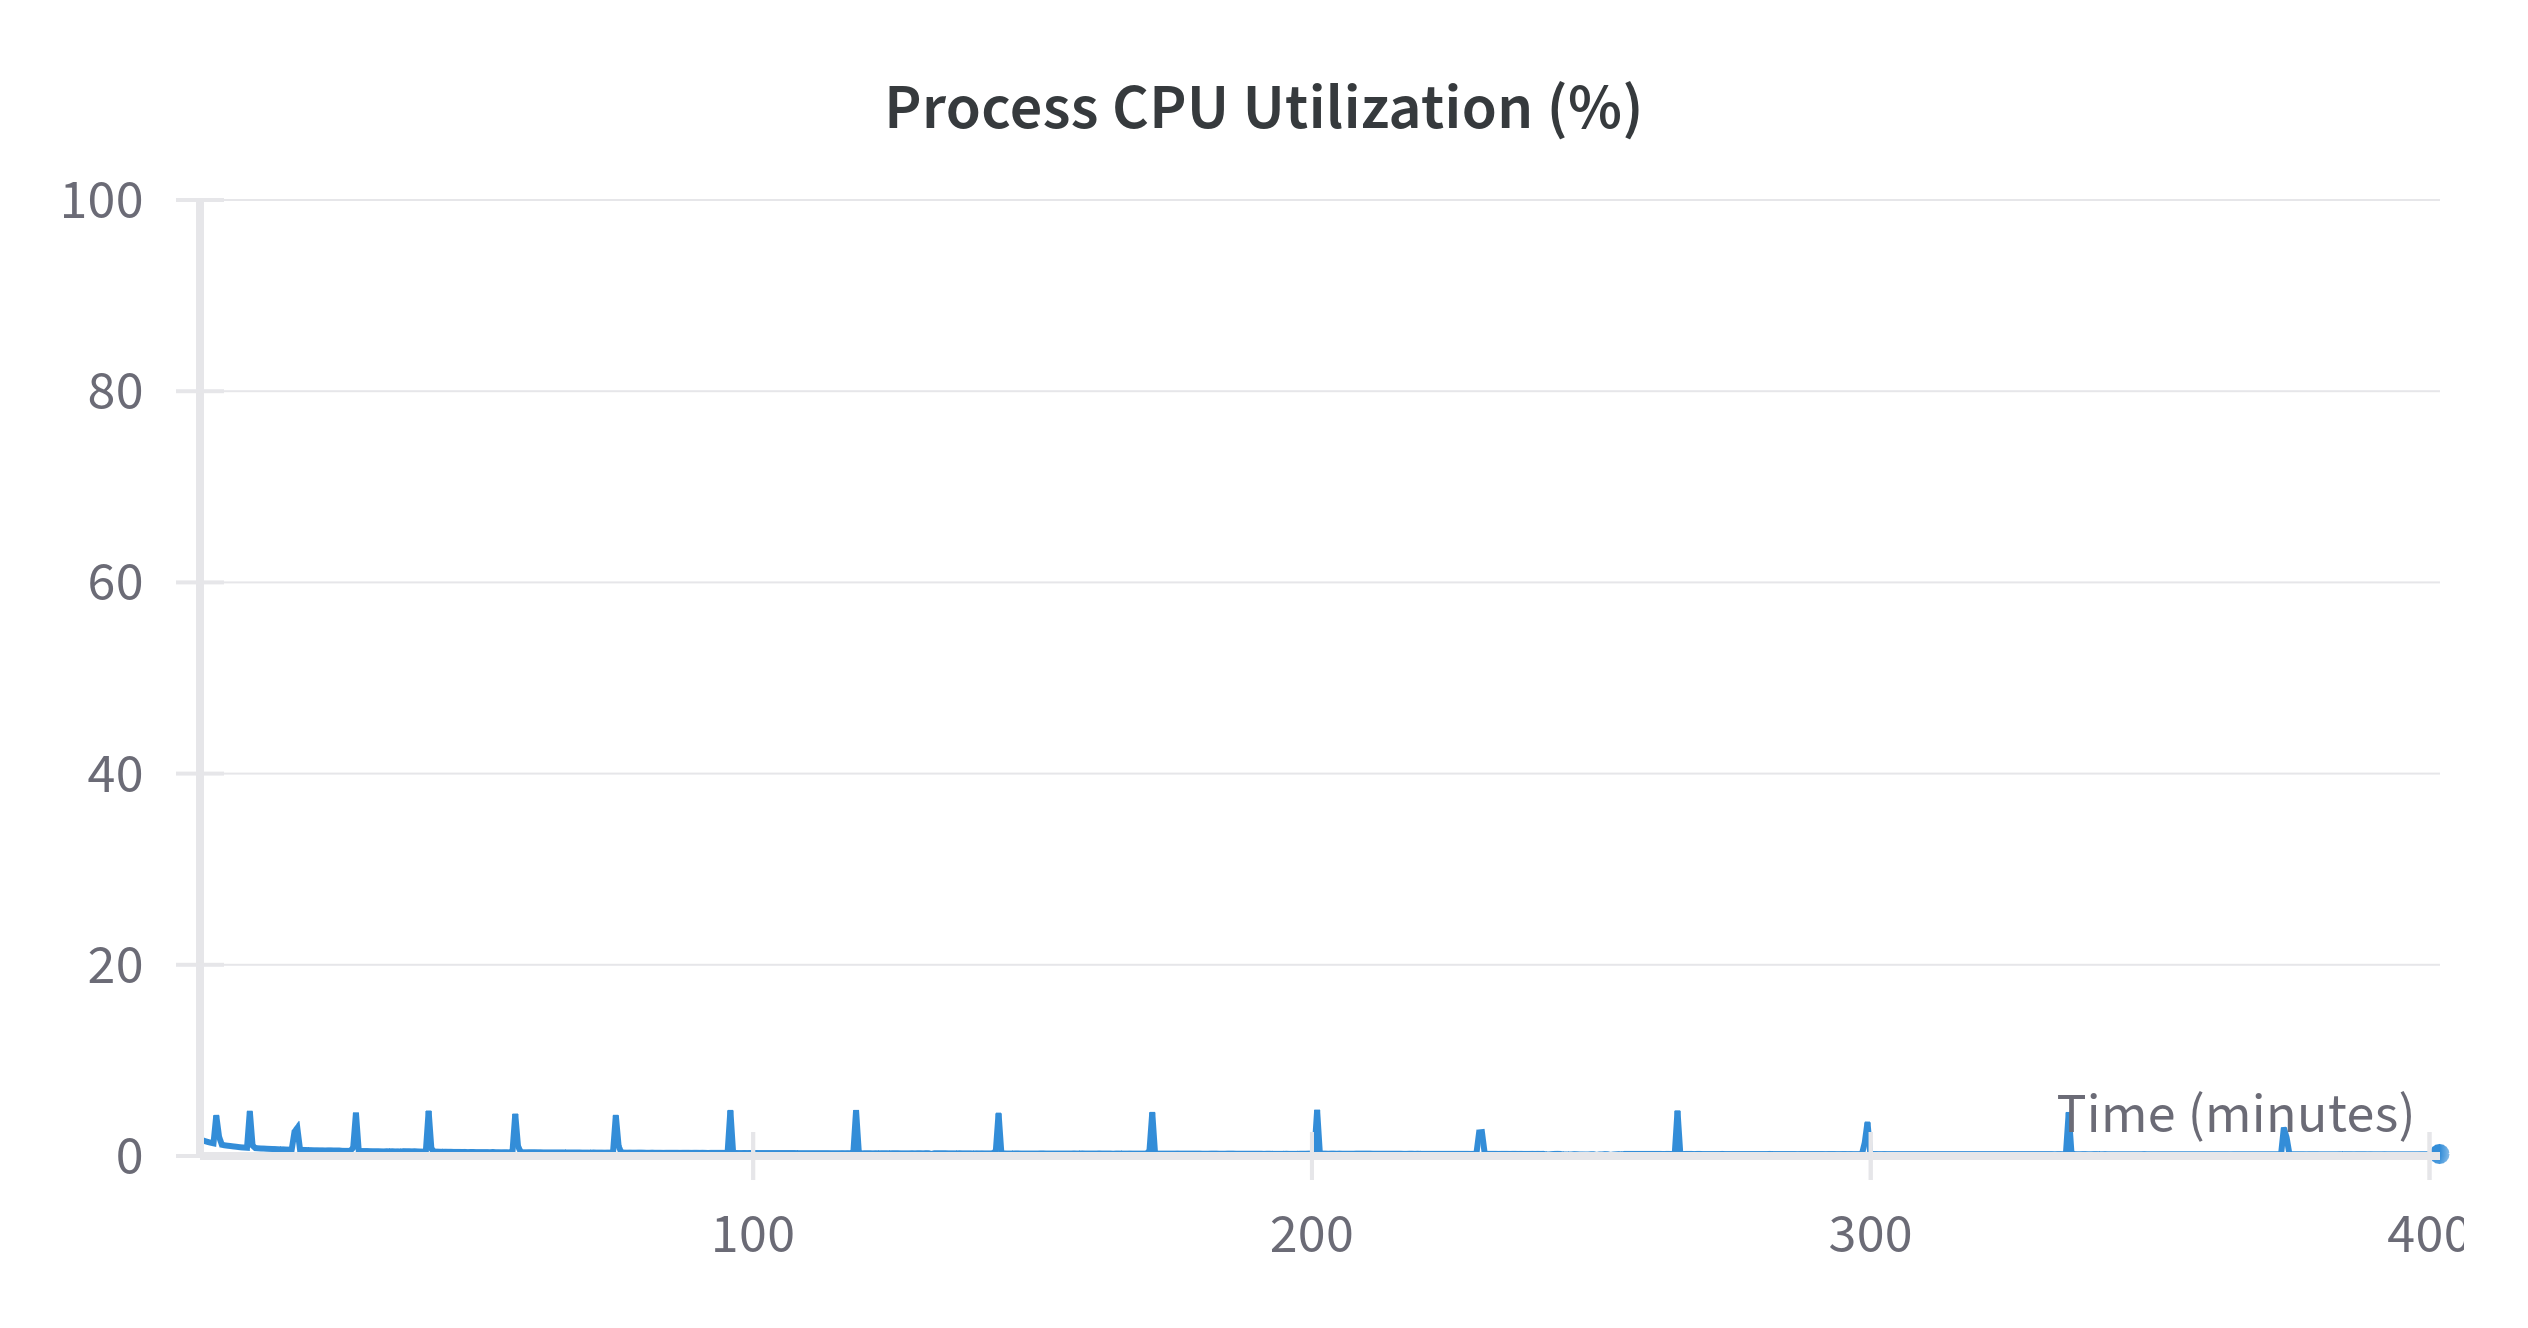
\includegraphics[width=0.8\textwidth]{figures/total_cpu_utilization.png}
    \caption{Total CPU usage while training an agent}
    \label{fig:ram_usage}
\end{figure}

\begin{figure}[H]
    \centering
    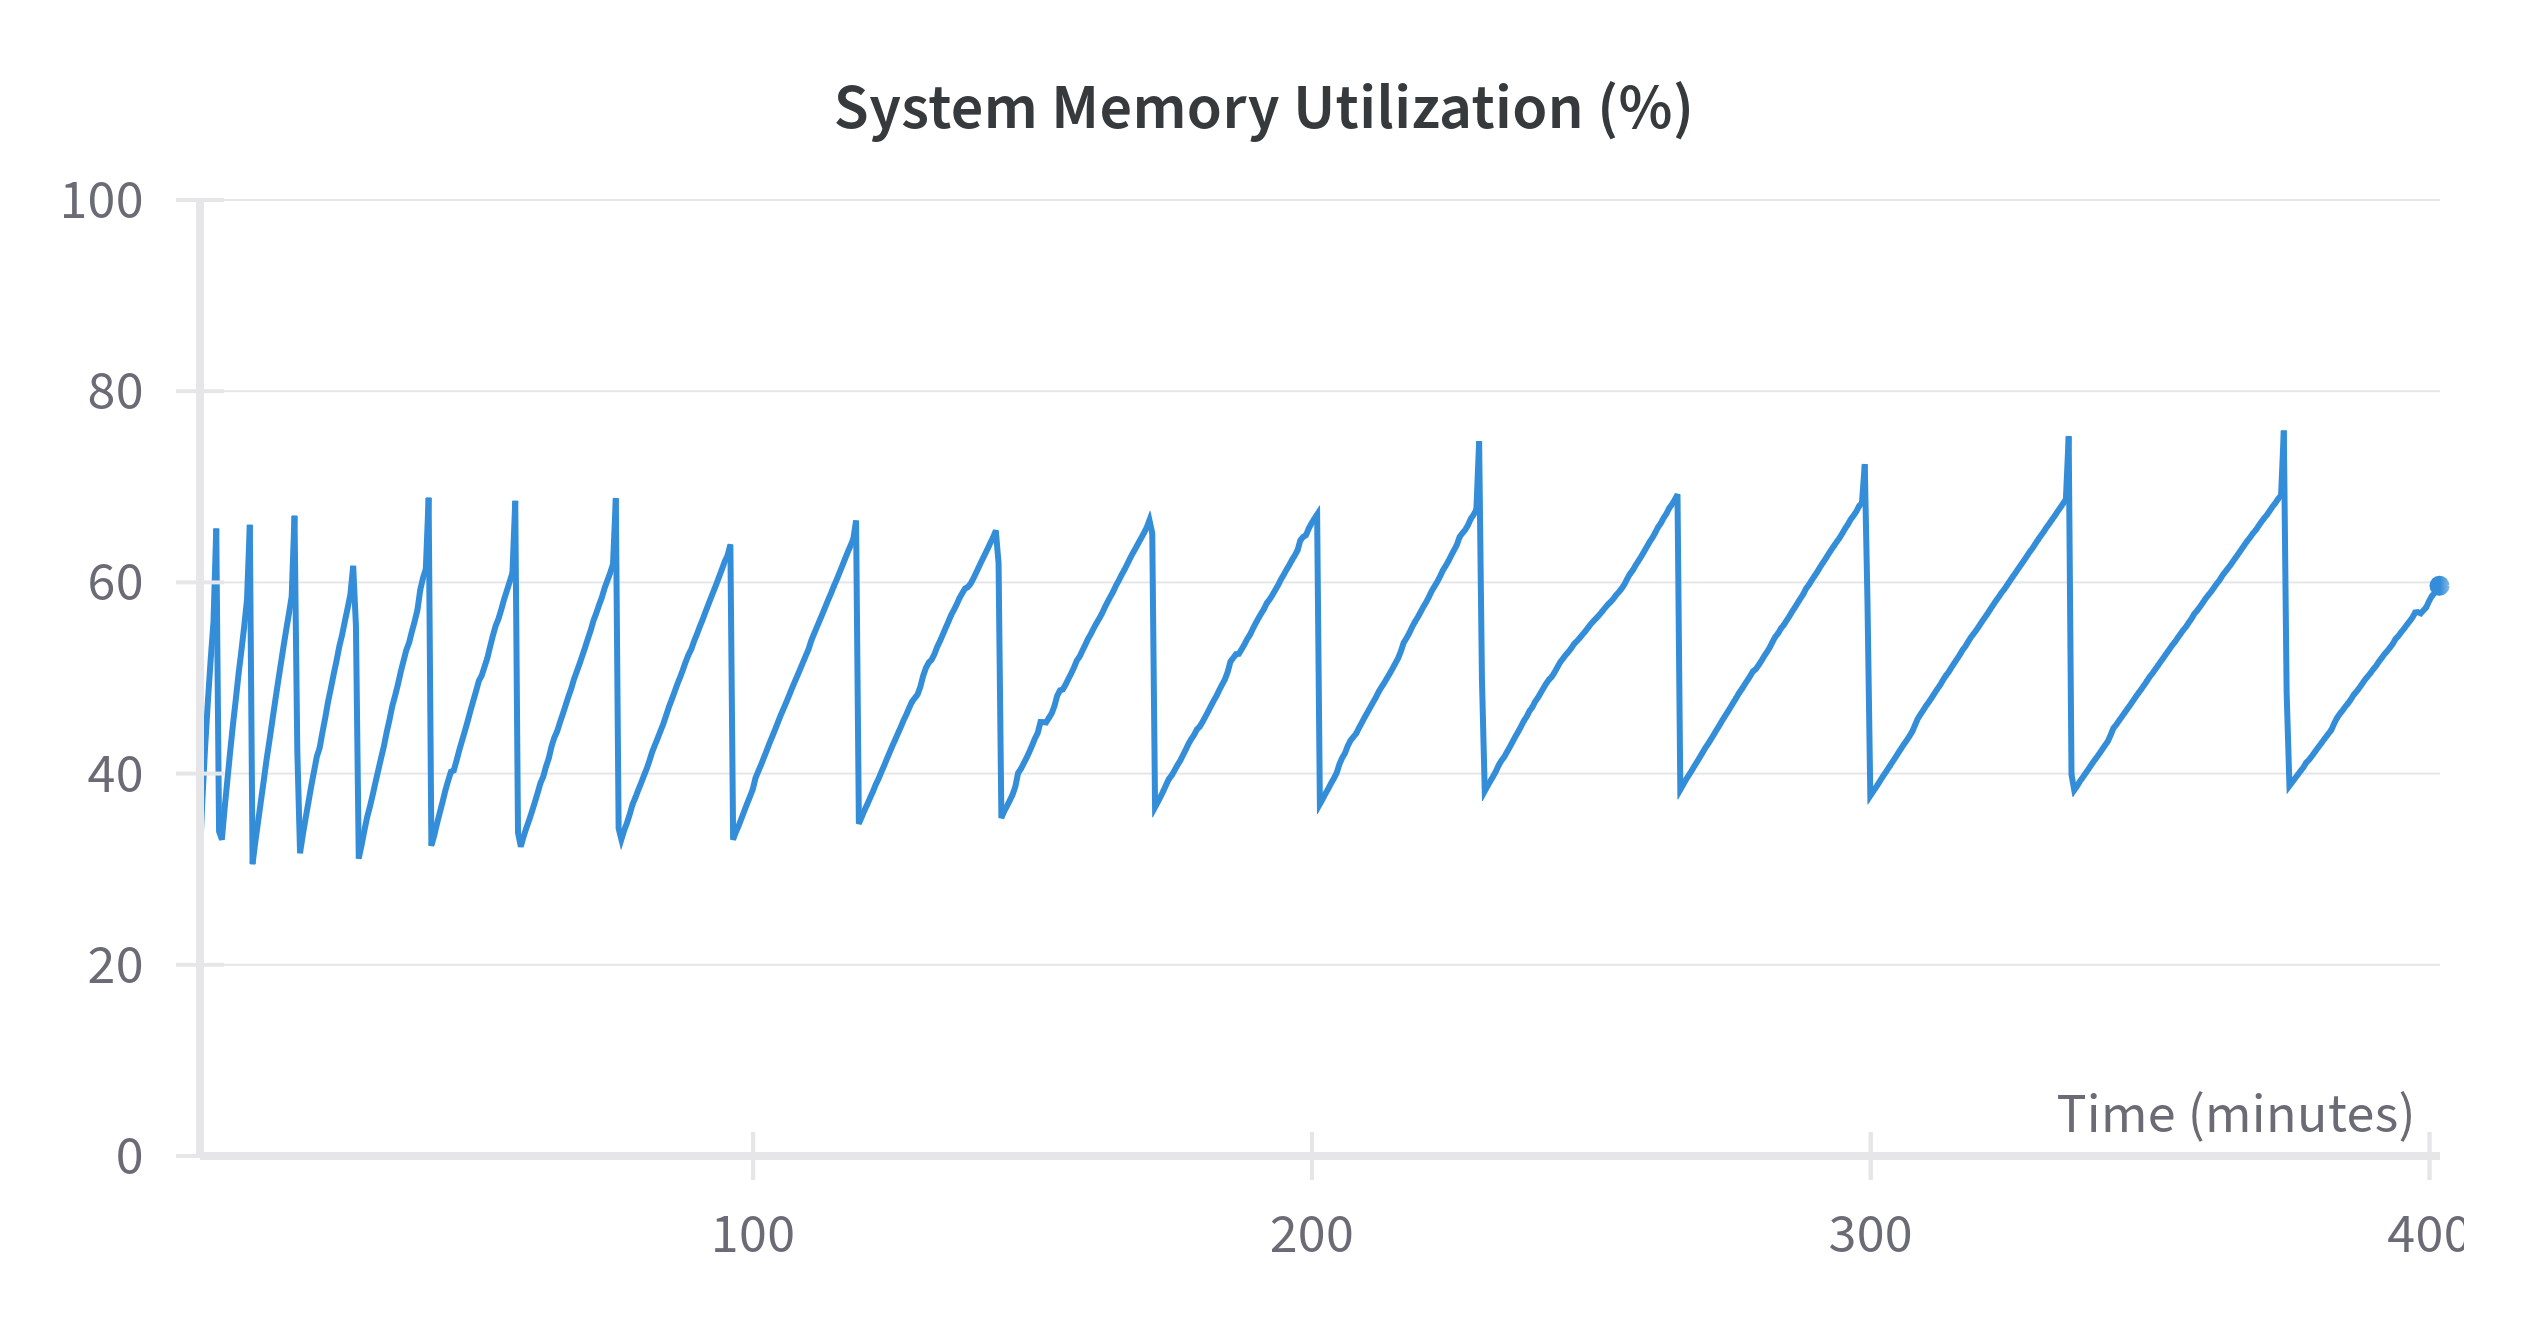
\includegraphics[width=0.8\textwidth]{figures/System_RAM_Utilization.png}
    \caption{Total RAM usage while training an agent}
    \label{fig:sys_memory_useage}
\end{figure}

From the three figures above, it can be seen that the GPU Utilization was low, with a maximum of 42.47\% peak usage. The CPU usage was also low, with a maximum of 4.71\% peak usage, while the Total RAM usage while training the agent was quite high, with a maximum of 75.82\% peak usage. The values provided in the figures above were taken from the wandb system monitor that was running while trianing the agents. In addition, these values have the possibility of being marginally skewed as the hardware running the training the agents was also running visual studio code and other system operating system essential processes. However, it is very evident that RAM was the bottleneck in training the agents. It was possible to train with an additional instance of the environment making the total instances 12, however there was a high chance that the system would crash. This occured while training the agent using the PPO algorithm after 4-5 hour. 

\subsection{Determining the optimal number of timesteps per episode}

Deciding on the total number of timesteps for each episode is a very difficult task to do as it is impossible to guage how many timesteps are needed for the agent to complete the first gym. The more timesteps per episode the more opportunities it has to explore the environment which would give it more potential options and paths it can take to find the optimal path with the given number of timesteps. However, the fewer timesteps per episode, the higher the risk that it is infeasible to complete the first gym and reward is maximized with the given number of timesteps, which would not include taking steps towards solving the problem of the environment. 

\subsection{Determning the optimzl training time}



\subsection{Data Recording}
